% Document class and parameters %
\documentclass[10pt,a4paper]{article}

% Document packages %
\usepackage{graphicx}
\usepackage{biblatex}
\usepackage{parskip}
\usepackage{listings}
\usepackage{caption}
\usepackage{subcaption}
\usepackage{amsmath}
\usepackage[most]{tcolorbox}

%%%%%%%%%%%%%%%%%%%%%%%%%%%%%%%%%%%%%%%%%%%%%%%%%%%%%%%%%%%%%%%%%%%%%%%%%%%%%%%%%%%%%%%%%%%%%%%%%%%%%%%%%%
% Parameters %
\lstset{basicstyle=\ttfamily, breaklines = true, tabsize=2}
\graphicspath{{./Images/}}
\setlength{\parskip}{1em}

%%%%%%%%%%%%%%%%%%%%%%%%%%%%%%%%%%%%%%%%%%%%%%%%%%%%%%%%%%%%%%%%%%%%%%%%%%%%%%%%%%%%%%%%%%%%%%%%%%%%%%%%%%

% Document Body %
\begin{document}
\begin{titlepage}
	\centering
	{\scshape\LARGE ELEC40001 \par}
	\vspace{1cm}
	{\scshape\Large Mathematics: Year 1\par}
	\vspace{1.5cm}
	{\huge\bfseries Independence, Basis and Dimension\par}
	\vspace{2cm}
	{\Large\ Xin Wang }
	\vfill
	{\large \today\par}
\end{titlepage}

\begin{abstract}
    Matrix calculations can be seen as only numbers. To engineers, it involves
    vectors i.e. columns of $A\textbf{x}$ and $AB$ are linear combinations of $n$ vectors - the columns 
    of $A$. Now matrix calculations are abstracted from numbers and vectors to a third highest level
    of understanding. Instead of individual columns, vector "spaces" are considered. Without 
    seeing vector spaces and their subspaces, everything cannot be understood about $A\textbf{x}= b$. 

    This section is about the true size of a subspace. There are $n$ columns in an $[m\times n]$
    matrix but the true \textbf{dimension} of the column space is not necessarily $n$.  The dimension is
    measured by counting \textbf{independent} columns - the true dimension of the column space is the rank $r$. 
    The idea of independence applies to any vectors in any vector space. Most of this section concentrates on the common subspaces such as the col­umn space and the nullspace of A.  
    
    The goal is to understand a \textbf{basis}: independent vectors that "span the space". 
\end{abstract}

%%%%%%%%%%%%%%%%%%%%%%%%%%%%%%%%%%%%%%%%%%%%%%%%%%%%%%%%%%%%%%%%%%%%%%%%%%%%%%%%%%%%%%%%%%%%%%%%%%%%%%%%%%

\tableofcontents
\pagebreak

%%%%%%%%%%%%%%%%%%%%%%%%%%%%%%%%%%%%%%%%%%%%%%%%%%%%%%%%%%%%%%%%%%%%%%%%%%%%%%%%%%%%%%%%%%%%%%%%%%%%%%%%%%

% Sections Body %
\section{Introduction}
%%%%%%%%%%%%%%%%%%%%%%%%%%%%%%%%%%%%%%%%%%%%%%%%%%%%%%%%%%%%%%%%%%%%%%%%%%%%%%%%%%%%%%%%%%%%%%%%%%%%%%%%%%
\subsection{Column Rank and Row Rank}

Given a matrix $A$ of dimension $[m\times n]$, there can be at most $n$ pivots because a column cannot have more than one pivot.

\begin{tcolorbox}[breakable,colback=white]
    \textbf{Full Row Rank}: Rank of $A$ is equal to the number of rows 
    $$
    r=m
    $$
    Column Space $C(A)$ is $R^m$ which is always solvable. 
\end{tcolorbox}

Full Row Rank properties:
\begin{itemize}
    \item All rows have pivots.
    \item $Ax=b$ has a solution for every right-sided $b$.
    \item Column space spans the whole space of $R^m$.
    \item There are $n-r=n-m$ special solutions in nullspace of $A$.
\end{itemize}

\begin{tcolorbox}[breakable,colback=white]
    \textbf{Full Column Rank}: Rank of $A$ is equal to the number of columns 
    $$
    r=n
    $$
    $n$ pivots with no free variables indicate that only $x=0$ is in the nullspace meaning that the
    columns are independent.
\end{tcolorbox}

Full Column Rank properties:
\begin{itemize}
    \item All columns of A are pivot columns.
    \item $A\textbf{x}=b$ can only have one solution or no solution.
    \item There are no free variables so no special solutions.
    \item The nullspace $N(A)$ contains only the zero vector.
\end{itemize}

Rank can be easily identified by finding the \textbf{Reduced Row Echelon Form} $R$. There are four
possible cases with $r$, $m$ and $n$:
\begin{itemize}
    \item $r=m=n$: Square matrix 
    $$A=\begin{bmatrix}
        1 & 2\\ 
        3 & 1
        \end{bmatrix} \sim 
        \begin{bmatrix}
        1 & 0\\ 
        0 & 1
        \end{bmatrix} = R = I$$
    \begin{itemize}
        \item $R$ is the Identity Matrix.
        \item $A$ is invertible.
        \item No free variables and nullspace is \textbf{only} the zero vector. 
        \item $A \textbf{x}=b$ always has a solution - an unique solution: $ \textbf{x}=A^{-1}b$.
        \item Rows are independent.
    \end{itemize}
    \item $r=m$ and $m<n$: Flat matrix (Full Row Rank)
    $$A=
    \begin{bmatrix}
    1 & 2 & 6 & 5\\ 
    0 & 1 & \frac{17}{5} & \frac{14}{5} 
    \end{bmatrix} \sim
    \begin{bmatrix}
    1 & 0 & -\frac{4}{5} & -\frac{3}{5}\\ 
    0 & 1 & \frac{17}{5} & \frac{14}{5}
    \end{bmatrix} = R$$
    \begin{itemize}
        \item There are $n-m=2$ free columns thus two free variables.
        \item Nullspace is the linear combination of $n-m$ special solution vectors.
        \item There are infinitely many solutions: $m_p + x_n$
    \end{itemize}
    \item $r=m$ and $m>n$: Tall matrix (Full Column Rank)
    $$A = \begin{bmatrix}
        1 & 3\\ 
        0 & 1\\ 
        0 & 0\\ 
        0 & 0
        \end{bmatrix} \sim
        \begin{bmatrix}
        1 & 0\\ 
        0 & 1\\ 
        0 & 0\\ 
        0 & 0
        \end{bmatrix} = R$$
    \begin{itemize}
        \item No free variables thus no special solutions.
        \item Columns are independent.
        \item One solution or, if $b$ is not in the column space, there is no solution.
    \end{itemize}
    \item $r<m$ and $r<n$: Not full rank
    \begin{itemize}
        \item $\infty$ solutions or $0$ if $b$ is not in the column space.
    \end{itemize}
\end{itemize}
\begin{tcolorbox}[breakable,colback=white]
    \centering
    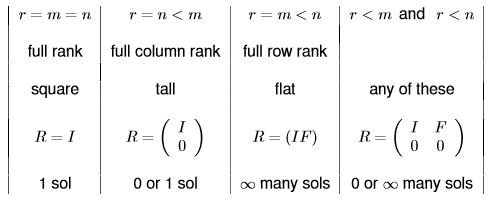
\includegraphics[scale=0.8]{Summary.JPG}
\end{tcolorbox}

%%%%%%%%%%%%%%%%%%%%%%%%%%%%%%%%%%%%%%%%%%%%%%%%%%%%%%%%%%%%%%%%%%%%%%%%%%%%%%%%%%%%%%%%%%%%%%%%%%%%%%%%%%
\subsection{Echelon form}

Echelon form of the matrix can be presented in two states:
\begin{itemize}
    \item Row echelon form.
    \item Reduced row echelon form.
\end{itemize}

This means that the matrix meets the following three requirements:
\begin{enumerate}
    \item The first number (leading coefficient) in the row is $1$.
    \item Every leading $1$ is to the right of the one above it.
    \item Any non-zero rows are always above rows with all zeros.
\end{enumerate}
\begin{figure} [h!]
    \centering
    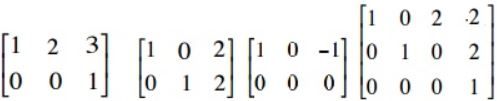
\includegraphics[scale=0.7]{Common echelon.JPG}
    \caption{Common examples of echelon form matrices}
\end{figure}

%%%%%%%%%%%%%%%%%%%%%%%%%%%%%%%%%%%%%%%%%%%%%%%%%%%%%%%%%%%%%%%%%%%%%%%%%%%%%%%%%%%%%%%%%%%%%%%%%%%%%%%%%%
\subsubsection{Row echelon form}

A matrix is in \textbf{row echelon form} if it meets the following requirements:
\begin{enumerate}
    \item The first non-zero number from the left is always to the right of the first non-zero number in the row above.
    \item Rows consisting of all zeros are at the bottom of the matrix.
\end{enumerate}
\begin{figure} [h!]
    \centering
    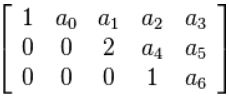
\includegraphics[scale=0.7]{row echelon form}
    \caption{Row echelon form}
\end{figure}

The row echelon form is used to determine basic matrix information such as \textbf{rank},
\textbf{free columns} and \textbf{identity columns}.

%%%%%%%%%%%%%%%%%%%%%%%%%%%%%%%%%%%%%%%%%%%%%%%%%%%%%%%%%%%%%%%%%%%%%%%%%%%%%%%%%%%%%%%%%%%%%%%%%%%%%%%%%%
\subsubsection{Reduced row echelon form}

Reduced row echelon form has four requirements:
\begin{enumerate}
    \item The first non-zero number in the first row is the number 1.
    \item The second row also starts with the number 1, which is further to the right than the leading entry in the first row. For every subsequent row, the number 1 must be further to the right.
    \item The leading entry in each row must be the only non-zero number in its column.
    \item Any non-zero rows are at the bottom of the matrix.
\end{enumerate}
\begin{figure} [h!]
    \centering
    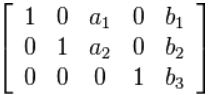
\includegraphics[scale=0.7]{reduced row echelon form.JPG}
    \caption{Reduced row echelon form}
\end{figure}

Reduced row echelon form is a type of matrix used to solve systems of linear equations. It is used
to find the \textbf{basis} and \textbf{dimension} of matrices.

%%%%%%%%%%%%%%%%%%%%%%%%%%%%%%%%%%%%%%%%%%%%%%%%%%%%%%%%%%%%%%%%%%%%%%%%%%%%%%%%%%%%%%%%%%%%%%%%%%%%%%%%%%
\section{Linear Independence}

\begin{tcolorbox}[breakable,colback=white]
    \textbf{Linear combination} (of $v_1, v_2,\dots,v_n$): There exists scalars defined as $x_1, x_2,\dots,x_n$
    such that the vector $v=(x_1 \times v_1)+(x_2 \times v_2)+\dots+(x_n \times v_n)$.
    \\
    \\
    \textbf{Linearly independence}: The only solution to $Ax=0$ is $x=0$ meaning the only
    combination that gives the zero vector is $0\:v_1 + 0\:v_2 + \dots + 0\:v_n$.
\end{tcolorbox}

In order for there to be linear independence between vectors, the vectors must not be in the same
plane. If the vectors are in the same plane then the vectors are \textbf{linearly dependent} so the
nullspace does not only contain the zero vector $N(A)\neq \textbf{\underbar 0}$. 
\begin{figure} [h!]
    \centering
    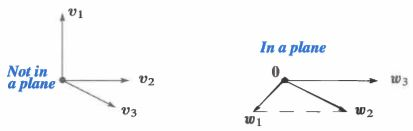
\includegraphics[scale=0.9]{Independence.JPG}
\end{figure}

\textbf{Example 1}: Columns of $A$ are dependent thus $Ax=0$ has a non-zero solution. 
\begin{equation*} 
    A=\begin{bmatrix}
        1 & 0 & 3\\ 
        2 & 1 & 5\\ 
        1 & 0 & 3
        \end{bmatrix} \textrm{ reduces to } R=\begin{bmatrix}
            1 & 0 & 3\\ 
            0 & 1 & -1\\ 
            0 & 0 & 0
            \end{bmatrix}
\end{equation*}
\begin{itemize}
    \item The rank is 2 so this means that there is a free column.
    \item Through Gaussian elimination, the special solution is a combination of the pivot columns.
\end{itemize}

\begin{tcolorbox}[breakable,colback=white]
    A easy way to check for linear independence is if the number of vector columns '$n$' is greater than
    number of vector rows '$m$'
    $$
        n<m
    $$
    
    If $n>m$ then the vector columns $R^m$ must be linearly dependent.
\end{tcolorbox}
\pagebreak

%%%%%%%%%%%%%%%%%%%%%%%%%%%%%%%%%%%%%%%%%%%%%%%%%%%%%%%%%%%%%%%%%%%%%%%%%%%%%%%%%%%%%%%%%%%%%%%%%%%%%%%%%%
\section{Vectors that 'Span' a Subspace}

\begin{tcolorbox}[breakable,colback=white,colframe=black,width=\dimexpr\textwidth+12mm\relax,enlarge left by=-6mm]
\textbf{Span}: A set of vectors \textit{span} a space if its linear combinations fill the space i.e. two vectors span a line, three could at best span all of $R^3$.
\end{tcolorbox}

There are two kinds of subspaces:
\begin{itemize}
    \item \textbf{Column subspace} $C(A)$ : Spans the Column Space i.e. contains all combinations of the
    columns of $A$ and is a subspace of $R^m$.
    \item \textbf{Row subspace} $C(A^T)$ : Spans the Row Space i.e. contains all combinations of the
    rows of $A$ and is a subspace of $R^m$.
\end{itemize}

\textbf{Example 1}: Describe the Column Space and Row Space of $A$.
\begin{equation*} 
    A=\begin{bmatrix}
        1 & 4 \\ 
        2 & 7 \\ 
        3 & 5 
        \end{bmatrix} \textrm{ and } A^T=\begin{bmatrix}
            1 & 2 & 3 \\ 
            4 & 7 & 5\\ 
            \end{bmatrix} \textrm{; m = 3 and n = 2}
\end{equation*}
\begin{enumerate}
    \item Find the $m$ and $n$.
    \begin{align*}
        m = 3 \; \text{ and } \; n=2
    \end{align*}
    \item Describe the Column Space with $m=3$.
    
    The Column Space spans two columns of $A$ thus is a plane in $R^3$.

    \item Describe the Row Space.
    
    The Row Space of $A$ spans three rows and spans all of $R^2$.
\end{enumerate}

%%%%%%%%%%%%%%%%%%%%%%%%%%%%%%%%%%%%%%%%%%%%%%%%%%%%%%%%%%%%%%%%%%%%%%%%%%%%%%%%%%%%%%%%%%%%%%%%%%%%%%%%%%
\subsection{Basis for a Vector Space}

A minimal set of vectors in $V$ that spans $V$ is called a \textbf{basis} for $V$. 

\begin{tcolorbox}[breakable,colback=white]
\textbf{Basis} (of a vector space): A sequence of vectors with the following properties:
\begin{itemize}
    \item All vectors are linearly independent i.e. a maximal linearly independent set.
    \item Span the entire space $V$.
\end{itemize} 
\end{tcolorbox}

\pagebreak

The properties of basis are important since every vector $v$ in vector space is \textbf{a unique combination
of basis vectors}. This means that \textbf{basis vectors are independent}. 

\begin{enumerate}
    \item Columns of all invertible $n \times n$ matrix give a basis for $R^n$. 
    \begin{center}
        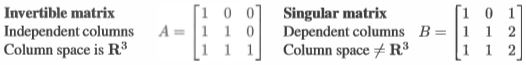
\includegraphics[scale=0.9]{Basis.JPG}
    \end{center}

    \item The \textbf{pivot columns} of $A$ are a \textbf{basis} for its column space and the \textbf{pivot rows}
    of $A$ are a basis for its row space. 

    \textbf{Example 1}: Given $c_1*\begin{bmatrix}
        1\\ 
        0\\ 
        0
        \end{bmatrix} + c_2*\begin{bmatrix}
            0\\ 
            1\\ 
            0
            \end{bmatrix}+c_3*\begin{bmatrix}
                0\\ 
                0\\ 
                1
                \end{bmatrix}$ does it form a basis? 
    The system form a Basis, the system spans the space $R^3$ and are linearly independent. 
\end{enumerate}

\textbf{Example 2}: Given vectors $\begin{bmatrix}
    1\\ 
    1\\ 
    1
    \end{bmatrix}$and $\begin{bmatrix}
        2\\ 
        3\\ 
        4
        \end{bmatrix}$ does it form a basis? If not, find a basis that includes the vectors.

\begin{enumerate}
    \item Note the linear combinations form a plane: 
    $$p*
    \begin{bmatrix}
        1\\ 
        1\\ 
        1
    \end{bmatrix} + q*
    \begin{bmatrix}
            2\\ 
            3\\ 
            4
    \end{bmatrix}
    $$

    \item Analyse the linear combination:
    \begin{itemize}
        \item The vectors are linearly independent since the vectors are not multiples of each other.
        \item Plane clearly does not span the entire $R^3$ so another independent vector is required.
    \end{itemize}

    \item Add a suitable vector to satisfy the conditions of a basis:
    $$
    c_1*\begin{bmatrix}
        1\\ 
        1\\ 
        1
        \end{bmatrix} + 
    c_2*\begin{bmatrix}
        2\\ 
        3\\ 
        4
        \end{bmatrix} + 
    c_3*\begin{bmatrix}
        3\\ 
        4\\ 
        6
        \end{bmatrix}
    $$

    \item Verify the conditions for a basis are met:
    \begin{itemize}
        \item A square matrix is produced.
        \item Linearly independent, there is a unique solution for $x=A^{-1}*b$.
        \item The system spans the entire $R^3$ hence forms a basis.
    \end{itemize}
\end{enumerate}

\begin{tcolorbox}[breakable,colback=white]
A simple test to ensure Linear Independence, simply find the Reduced Row Echelon form of the matrix.
\end{tcolorbox}

%%%%%%%%%%%%%%%%%%%%%%%%%%%%%%%%%%%%%%%%%%%%%%%%%%%%%%%%%%%%%%%%%%%%%%%%%%%%%%%%%%%%%%%%%%%%%%%%%%%%%%%%%%
\section{Dimension}

\begin{tcolorbox}[breakable,colback=white]
\textbf{Dimension} (of a space): The number of vectors in a basis. 
For example, $R^3$ has 3 as a dimension and $R^2$ has 2 as a dimension.
\end{tcolorbox}
Theorems: 
\begin{itemize}
    \item Dimension of column space is equal to the rank of the matrix
    $$rank(A)=dimC(A)$$
    \item Dimension of nullspace of $m\times n$ matrix is equal to number of columns minus the rank
    $$n-rank(A)=dimN(A)$$
    \item Existence of solution of $Ax=b$:
    \begin{itemize}
        \item $Ax=b$ has a solution for all $b$
        \item Column space of $A$ is the entire $R^m$
        \item rank(A)=m
        \item Full Row Rank - Rows are linearly independent
        \item If $m=n$, rows of $A$ form the basis
    \end{itemize}
    \item Uniqueness of solution of $Ax=b$:
    \begin{itemize}
        \item If $Ax=b$ has a solution, it is unique
        \item Nullspace contains only the Zero Vector
        \item $rank(A)=n$
        \item Columns are linearly independent (Full Column Rank)
        \item If $m=n$, rows of $A$ form the basis
    \end{itemize}
\end{itemize}
\pagebreak 

%%%%%%%%%%%%%%%%%%%%%%%%%%%%%%%%%%%%%%%%%%%%%%%%%%%%%%%%%%%%%%%%%%%%%%%%%%%%%%%%%%%%%%%%%%%%%%%%%%%%%%%%%%
\section{The Four Fundamental Subspaces}

\textbf{Rank} i.e. number of pivots and \textbf{dimension} i.e. number of vectors in a basis are
important terms used to describe the four fundamental subspaces. Those subspaces are the column
space and the nullspace of $A$ and $A^T$. Together, they lift the understanding of $A \textbf{x}=b$
to a higher level - the subspace level.

They are all connected by the Fundamental Theorem of Linear Algebra.  The four fundamental subspaces are:
\begin{itemize}
    \item Column space $C(A)$ of $A$ - The subspace of $\Re^m$ spanned by the columns of $A$. 
    \item Row space $C(A^T)$ of $A$ - The subspace of $\Re^n$ spanned by the rows of $A$.
    \item Nullspace $N(A)$ of $A$ - The subspace of $\Re^n$ of solutions of $Ax=0$.
    \item Left Nullspace $N(A^T)$ of $A$ - The subspace of $\Re^m$ of solutions of $A^T x = 0$
\end{itemize}

\begin{figure} [h!]
    \centering
    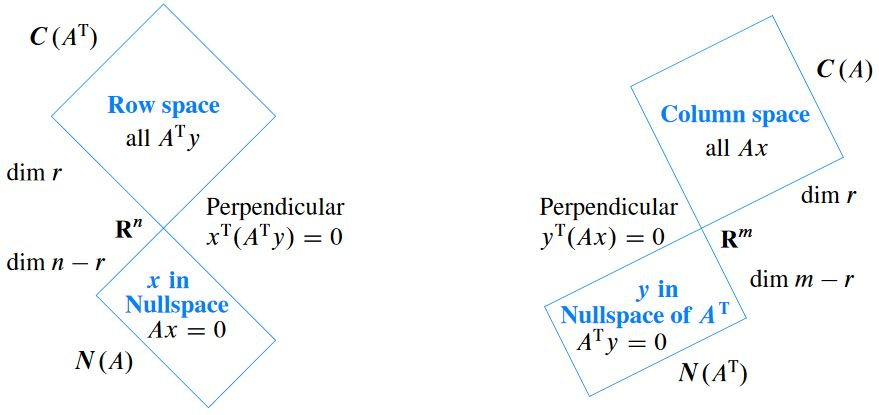
\includegraphics[scale=0.6]{Fundasub.JPG}
    \caption{Dimensions and orthogonality for any $m$ by $n$ matrix $A$ of rank $r$.}
\end{figure}

%%%%%%%%%%%%%%%%%%%%%%%%%%%%%%%%%%%%%%%%%%%%%%%%%%%%%%%%%%%%%%%%%%%%%%%%%%%%%%%%%%%%%%%%%%%%%%%%%%%%%%%%%%
\subsection{The basis and dimension of the Four Fundamental Subspaces}

\begin{tcolorbox}[breakable,colback=white]
\textbf{Tip}: Always obtain the Reduce Row Echelon Form of a given matrix before finding the four bases.
\end{tcolorbox}

Finding the basis of these vector spaces to determine the dimensions are important to understanding
the four fundamental subspaces.

\pagebreak
%%%%%%%%%%%%%%%%%%%%%%%%%%%%%%%%%%%%%%%%%%%%%%%%%%%%%%%%%%%%%%%%%%%%%%%%%%%%%%%%%%%%%%%%%%%%%%%%%%%%%%%%%%
\subsubsection{Column space $C(A)$:}

Note that elementary row operations do change the column space and it is not obvious that $\text{dim
}C(A)=\text{dim }C(A^T)$ [See: Proof of column space dimension]. The columns of $U$ that contain the
pivots are  linearly  independent and the corresponding columns of $A$ are also linearly
independent. The other dependent columns of $A$ are dependent on the independent columns thus they
will also span $C(A)$. This means that the independent columns i.e. pivot columns form a basis for
this space. 

As the dimension is the number of number of independent variables:
$$
    \text{dim }C(A) = r
$$

\begin{tcolorbox}[breakable,colback=white]
    For the column space $C(A)$ by expressing it in reduced row echelon form.:
    \begin{enumerate}
        \item Basis: Number of independent variables i.e. pivot columns.
        \item Dimension: The rank of $A$ defined as $\text{dim }C(A)= \text{rank}(A) = r$ 
    \end{enumerate}
\end{tcolorbox}

%%%%%%%%%%%%%%%%%%%%%%%%%%%%%%%%%%%%%%%%%%%%%%%%%%%%%%%%%%%%%%%%%%%%%%%%%%%%%%%%%%%%%%%%%%%%%%%%%%%%%%%%%%
\subsubsection{Row space $C(A^T)$}

If $B$ is obtained from $A$ by elementary row operations, then the rows of $B$ are \textbf{linear combinations} 
of  the rows of $A$. Since the elementary row operations can all be reversed, the rows of $A$ are also
linear combinations of the rows of $B$
$$
    C(A^T) = C(B^T)
$$

Building on, taking $A$ to its row echelon form $U$ by elementary row operations, the non-zero rows
of $U$ form a basis for the row space of $U$ and hence for the row space of A. By finding the basis
and letting $r = \text{rank}(A)$, the dimension is defined as:
$$
    \text{dim}\: C(A^T) = r
$$

\begin{tcolorbox}[breakable,colback=white]
For the row space $C(A^T)$ by expressing it in reduced row echelon form.:
\begin{enumerate}
    \item Basis: Number of independent variables i.e. non-zero rows.
    \item Dimension: The rank of $A$ defined as $\text{dim }C(A^T)= \text{rank}(A)$ 
\end{enumerate}
\end{tcolorbox}

%%%%%%%%%%%%%%%%%%%%%%%%%%%%%%%%%%%%%%%%%%%%%%%%%%%%%%%%%%%%%%%%%%%%%%%%%%%%%%%%%%%%%%%%%%%%%%%%%%%%%%%%%%
\subsubsection{Nullspace $N(A)$:}

Notice that elementary row operations do not change this space at all i.e. if $A$ is expressed in
$A=LU$ through Gaussian elimination to find the nullspace, the lower triangular $L$ will have all
its diagonal coefficients equal to 1. This means that with the definition of the nullspace $Ax=0$:
$$
    Ax=0 \Leftrightarrow (LU)x=0 \Leftrightarrow L^{-1}LUx=L^{-1}0=0
$$
Allowing $Ax = 0$ to be simplified to:
$$
    Ax = 0 \Leftrightarrow Ux = 0
$$

Then, a basis for $N(A)$ is actually a basis for $N(U)$ which is \textbf{the number of free variables
present in the system $Ux=0$}.

If $\text{rank}(A)=r$ and the number of variables is $n$, then the number of pivots is $r$ and the
number of free variables is $n-r$ thus the dimension of the null space is defined as:
$$
    \text{dim}\: N(A) = n - r
$$

\textbf{Example 1}: Given a matrix $A$ already expressed in echelon form to find $U$, find the
special solutions thus a basis and dimension.
\begin{align*}
    \begin{bmatrix}
        1&2&2&2 \\ 
        0&0&2&4 \\
        0&0&0&0 
    \end{bmatrix} 
    \begin{bmatrix}
        x_1 \\
        x_2 \\
        x_3 \\
        x_4 
    \end{bmatrix} = 0
\end{align*}
Process:
\begin{enumerate}
    \item Identify the \textbf{free columns} (2 and 4) and \textbf{pivot columns} (1 and 3).
    \item Assign any value to the 2 free variables to find the 2 special solutions:
    \begin{itemize}
        \item $x_2=1$ and $x_4=0$
        \begin{align*}
            2x_3+4x_4=0 &\Rightarrow x_3=0 \\
            x_1+2x_2+2x_3+2x_4=0 &\Rightarrow x_1=-2
        \end{align*}
        Thus solution 1 is:
        \begin{align*}
            x = 
            \begin{bmatrix}
                -2 \\
                1 \\
                0 \\
                0
            \end{bmatrix}    
        \end{align*}
        \item $x_2=0$ and $x_4=1$
        \begin{align*}
            2x_3+4x_4 = 0 &\Rightarrow x_3 = -2 \\
            x_1+2x_2+2x_3+2x_4=0 &\Rightarrow x_1=2
        \end{align*}
        Thus solution 2 is:
        \begin{align*}
            x = 
            \begin{bmatrix}
                2 \\
                0 \\
                -2 \\
                1
            \end{bmatrix}    
        \end{align*}
    \end{itemize}
    \item Find the basis:
    \begin{align*}
        \text{A basis of null space: } \begin{bmatrix}
            -2 \\
            1 \\
            0 \\
            0
        \end{bmatrix} \; \text{ and } \;
        \begin{bmatrix}
            2 \\
            0 \\
            -2 \\
            1
        \end{bmatrix}
    \end{align*}
    \item Find the dimension:
    \begin{align*}
        \text{dim}\: N(A) = n - r \Rightarrow \text{dim}\: N(A) = 4 - 1 = 3
    \end{align*}
\end{enumerate}

\begin{tcolorbox}[breakable,colback=white]
    For the null space $N(A)$ by expressing it in reduced row echelon form.:
    \begin{enumerate}
        \item Basis: The number of free variables present in the system $Ux=0$.
        \item Dimension: The difference between the number of columns $n$ and the rank $r$ of $A$ is the same as the number of pivots:
        $$
            \text{dim}\: N(A) = n - r
        $$
    \end{enumerate}
\end{tcolorbox}

%%%%%%%%%%%%%%%%%%%%%%%%%%%%%%%%%%%%%%%%%%%%%%%%%%%%%%%%%%%%%%%%%%%%%%%%%%%%%%%%%%%%%%%%%%%%%%%%%%%%%%%%%%
\subsubsection{Left null space $N(A^T)$:}

If $A$ is $[m \times n]$ then $A^T$ is $[n \times m]$ and left null space is a subspace of $\Re^n$.
For the left null space $N(A^T)$, it is clear that since $\text{rank}(A)=\text{rank}(A^T)$:
$$
    \text{dim }N(A^T) = m-r
$$

A basis for $N(A^T)$ is found by using $A^T$ in its row echelon form and using the free variables to
find the basis vectors like the with the null space $N(A)$ i.e. giving each free variable in turn
the value 1 while all other independent variables take the value 0.

If it is observed that $R$ has no zero rows then there is no combination of the rows of $A$ that
gives a row of zeroes, i.e. there is no $y$ such that
$$
\textbf{\underline{y}}^T A = \textbf{\underline{0}}^T
$$
This means that there is only the zero vector as solution, so the only vector in the left null-space is 0, and it is the basis.

\textbf{Example 1}: Find a basis and the dimensions of the left null space of $A$:
\begin{align*}
    A = \begin{bmatrix}
        0&2&3&4 \\
        0&6&7&8 \\
        0&10&11&12
    \end{bmatrix}  
    \Rightarrow 
    A^T = \begin{bmatrix}
        0&0&0 \\
        2&6&10 \\
        3&7&11 \\
        4&8&12
    \end{bmatrix}
\end{align*}
Process:
\begin{enumerate}
    \item Find the row echelon form of $A^T$:
    \begin{align*}
        \begin{bmatrix}
            0&0&0 \\
            2&6&10 \\
            3&7&11 \\
            4&8&12
        \end{bmatrix}
        \Rightarrow
        \begin{bmatrix}
            \textbf{2}&6&10 \\
            0&-2&-4 \\
            0&-4&-8 \\
            0&0&0 
        \end{bmatrix}
        \Rightarrow
        \begin{bmatrix}
            \textbf{2}&6&10 \\
            0&\textbf{-2}&-4 \\
            0&0&0 \\
            0&0&0
        \end{bmatrix}
    \end{align*}
    \item Find the dimension:
    \begin{align*}
        \text{dim }N(A^T) = 3 -2 = 1
    \end{align*}
    \item Note that only one non-zero vector $x$ such that $A^Tx=0$ is needed since the dimension is
    $1$
    \item Find the special solution of $A^T$:
    \begin{itemize}
        \item One free variable $x_3$
        \item Set $x_3 = 1$
        \begin{align*}
            -2(x_2) -4(x_3) =0 \Rightarrow x_2 = -2
        \end{align*}
        \item Find all the unknown variables:
        \begin{align*}
            2x_1 + 6x_2 + 10x_3 = 0 \Rightarrow x_1 = 1
        \end{align*}
    \end{itemize}
    \item Form the basis from the special solutions:
        \begin{align*}
            \text{Basis for } N(A^T): 
            \begin{bmatrix}
                1 \\
                -2 \\
                1
            \end{bmatrix}
        \end{align*}
\end{enumerate}

\begin{tcolorbox}[breakable,colback=white]
    For the left null space $N(A^T)$ by expressing it in reduced row echelon form.:
    \begin{enumerate}
        \item Basis: The number of free variables present in the system $Ux=0$.
        \item Dimension: The difference between the number of columns $n$ and the rank $r$ of $A$ is the same as the number of pivots:
        $$
            \text{dim}\: N(A) = m - r
        $$
    \end{enumerate}
\end{tcolorbox}

\pagebreak
%%%%%%%%%%%%%%%%%%%%%%%%%%%%%%%%%%%%%%%%%%%%%%%%%%%%%%%%%%%%%%%%%%%%%%%%%%%%%%%%%%%%%%%%%%%%%%%%%%%%%%%%%%
\subsection{Examples}

\textbf{Example 1}: Given the matrix $A$, find a basis for each of the four fundamental subspaces
$C(A)$, $N(A)$, $C(A^T)$ and $N(A^T)$. Verify the relations linking the dimensions of the subspaces
to the size of the matrix $m \times n$ and rank $r$.
\begin{align*}
    A = 
    \begin{bmatrix}
        0&1&2&3 \\
        1&2&3&4 \\
        1&1&1&2
    \end{bmatrix}
\end{align*}

Process:
\begin{enumerate}
    \item Column space $C(A)$:
    \begin{itemize}
        \item Basis:
        \begin{itemize}
            \item Note: A basis is formed by pivot columns 
            \item Find the echelon form:
            \begin{align*}
                \text{Echelon form} = 
                \begin{bmatrix}
                    \textbf{1}&0&-1&0 \\
                    0&\textbf{1}&2&2 \\
                    0&0&0&\textbf{1}
                \end{bmatrix}
            \end{align*}
            \item Select the pivot columns.
            \begin{align*}
                \text{A basis for }C(A) = 
                \begin{bmatrix}
                    0 \\
                    1 \\
                    1
                \end{bmatrix}, \: 
                \begin{bmatrix}
                    1 \\
                    2 \\
                    1
                \end{bmatrix}, \:
                \begin{bmatrix}
                    3 \\
                    4 \\
                    2
                \end{bmatrix}
            \end{align*}
        \end{itemize}
        \item Dimension:
        \begin{itemize}
            \item $\text{dim }C(A) = r = \text{number of pivot columns}$
            \begin{align*}
                \text{dim }C(A) = r = 3
            \end{align*}
        \end{itemize}
    \end{itemize}
    \item Null space $N(A)$:
    \begin{itemize}
        \item Basis:
        \begin{itemize}
            \item Note: A basis is formed by special solutions
            \item Find the echelon form:
            \begin{align*}
                \text{Echelon form} = 
                \begin{bmatrix}
                    \textbf{1}&0&-1&0 \\
                    0&\textbf{1}&2&2 \\
                    0&0&0&\textbf{1}
                \end{bmatrix}
            \end{align*}
            \item Find the number of special solutions:
            \begin{align*}
                \text{Number of special solutions}=\text{Number of free columns}=1
            \end{align*}
            \item Set $x_3 = 1$ and find the values of the other variables:
            \begin{align*}
                x_3 &= 1 \\
                x_4 &= 0 \\
                x_1 &= x_3 = 1 \\
                x_2 &= -2x_3 = -2
            \end{align*}
            \item Find the special solution thus a basis for $N(A)$:
            \begin{align*}
                N(A) = p
                \begin{bmatrix}
                    1 \\
                    -2 \\
                    1 \\
                    0
                \end{bmatrix}
            \end{align*}
        \end{itemize}
        \item Dimension:
        \begin{itemize}
            \item $\text{dim }C(A) = n-r$
            \begin{align*}
                \text{dim }C(A) = n-r = 4-3 = 1
            \end{align*}
        \end{itemize}
    \end{itemize}
    \item Row space $C(A^T)$:
    \begin{itemize}
        \item Basis:
        \begin{itemize}
            \item Note: A basis is formed by special solutions
            \item Find the reduced echelon form of $A$:
            \begin{align*}
                \text{Reduced echelon form of }A = 
                \begin{bmatrix}
                    \textbf{1}&0&-1&0 \\
                    0&\textbf{1}&2&0 \\
                    0&0&0&\textbf{1}
                \end{bmatrix}
            \end{align*}
            \item Find the reduced echelon form of $A^T$:
            \begin{align*}
                \text{Reduced echelon form of }A^T = 
                \begin{bmatrix}
                    \textbf{1}&0&0 \\
                    0&\textbf{1}&0 \\
                    -1&2&0 \\
                    0&0&\textbf{1}
                \end{bmatrix}
            \end{align*}
            \item Find the number of special solutions:
            \begin{align*}
                \text{Number of special solutions}=\text{Number of pivot columns}=3
            \end{align*}
            \item Find the basis by listing the pivot columns:
            \begin{align*}
                \text{A basis for }C(A^T) = 
                \begin{bmatrix}
                    1 \\
                    0 \\
                    -1 \\
                    0
                \end{bmatrix}, \: 
                \begin{bmatrix}
                    0 \\
                    1 \\
                    2 \\
                    0
                \end{bmatrix}, \:
                \begin{bmatrix}
                    0 \\
                    0 \\
                    0 \\
                    1
                \end{bmatrix}
            \end{align*}
        \end{itemize}
        \item Dimension:
        \begin{itemize}
            \item $\text{dim }C(A) = n-r$
            \begin{align*}
                \text{dim }C(A) = r = 3 
            \end{align*}
        \end{itemize}
    \end{itemize}
    \item Left null space $N(A^T)$: 
    \begin{itemize}
        \item Basis:
        \begin{itemize}
            \item Note: A basis is the number of zero rows.
            \item Find the reduced echelon form of $A$:
            \begin{align*}
                \text{Reduced echelon form of }A = 
                \begin{bmatrix}
                    \textbf{1}&0&-1&0 \\
                    0&\textbf{1}&2&0 \\
                    0&0&0&\textbf{1}
                \end{bmatrix}
            \end{align*}
            \item Find the reduced echelon form of $A^T$:
            \begin{align*}
                \text{Reduced echelon form of }A^T = 
                \begin{bmatrix}
                    \textbf{1}&0&0 \\
                    0&\textbf{1}&0 \\
                    -1&2&0 \\
                    0&0&\textbf{1}
                \end{bmatrix}
            \end{align*}
            \item Identify number of zero rows to determine special solutions:
            \begin{align*}
                \text{Number of zero rows} = \text{Number of special solutions} = 0
            \end{align*}
        \end{itemize}
        \item Dimension:
        \begin{itemize}
            \item $\text{dim }C(A) = m-r$
            \begin{align*}
                \text{dim }C(A) = m-r = 3-3 = 0
            \end{align*}
        \end{itemize}
    \end{itemize}
\end{enumerate}



%%%%%%%%%%%%%%%%%%%%%%%%%%%%%%%%%%%%%%%%%%%%%%%%%%%%%%%%%%%%%%%%%%%%%%%%%%%%%%%%%%%%%%%%%%%%%%%%%%%%%%%%%%
\end{document}